\section*{Results}


The preliminary results point to some interesting dynamics. 40\% of respondents view China as having both ``A lot'' of influence and ``Somewhat positive'' or ``Very positive'' influence. Similarly, around 44\% of respondents view the United States as having ``A lot'' of influence in Kenya and view that influence as ``Somewhat positive'' or ``Very positive.'' Regarding military deployments, only 20\% of Kenya respondents believed that China has military personnel operating in Kenya, compared with 72\% of respondents who correctly responded that the United States has military personnel deployed to Kenya. Of those correctly identifying a Chinese military presence in Kenya, 63\% viewed that presence as ``Very positive'' or ``Somewhat positive.'' Similarly, of those correctly identifying a U.S. military presence in Kenya, 70\% % viewed that presence favorably. Figure 1 shows the joint distribution of respondents' answers to the questions about the presence of deployments and their evaluations of those deployments. 




These preliminary results suggest that public views of these major powers are comparable and potentially well-positioned for competitive influence campaigns. However, the United States and China also proceed from different starting points. A 2023 U.S. Department of Defense report notes that China's People's Liberation Army Strategic Support Force has limited personnel operating in Kenya. It expects China's pursuit of basing access to grow (DoD 2023). The United States has relatively high favorability levels and a long track record of basing in foreign countries. Given its relatively small military footprint to date, it remains to be seen if China can sustain such high levels of public approval as it expands the scope of its military-basing activities. Understanding the factors that shape public assessments of the costs and benefits of foreign basing will be key to understanding how this process will play out for the United States and China as they compete for access.


\begin{figure}[t]
	\begin{center}
		\scalebox{.6}{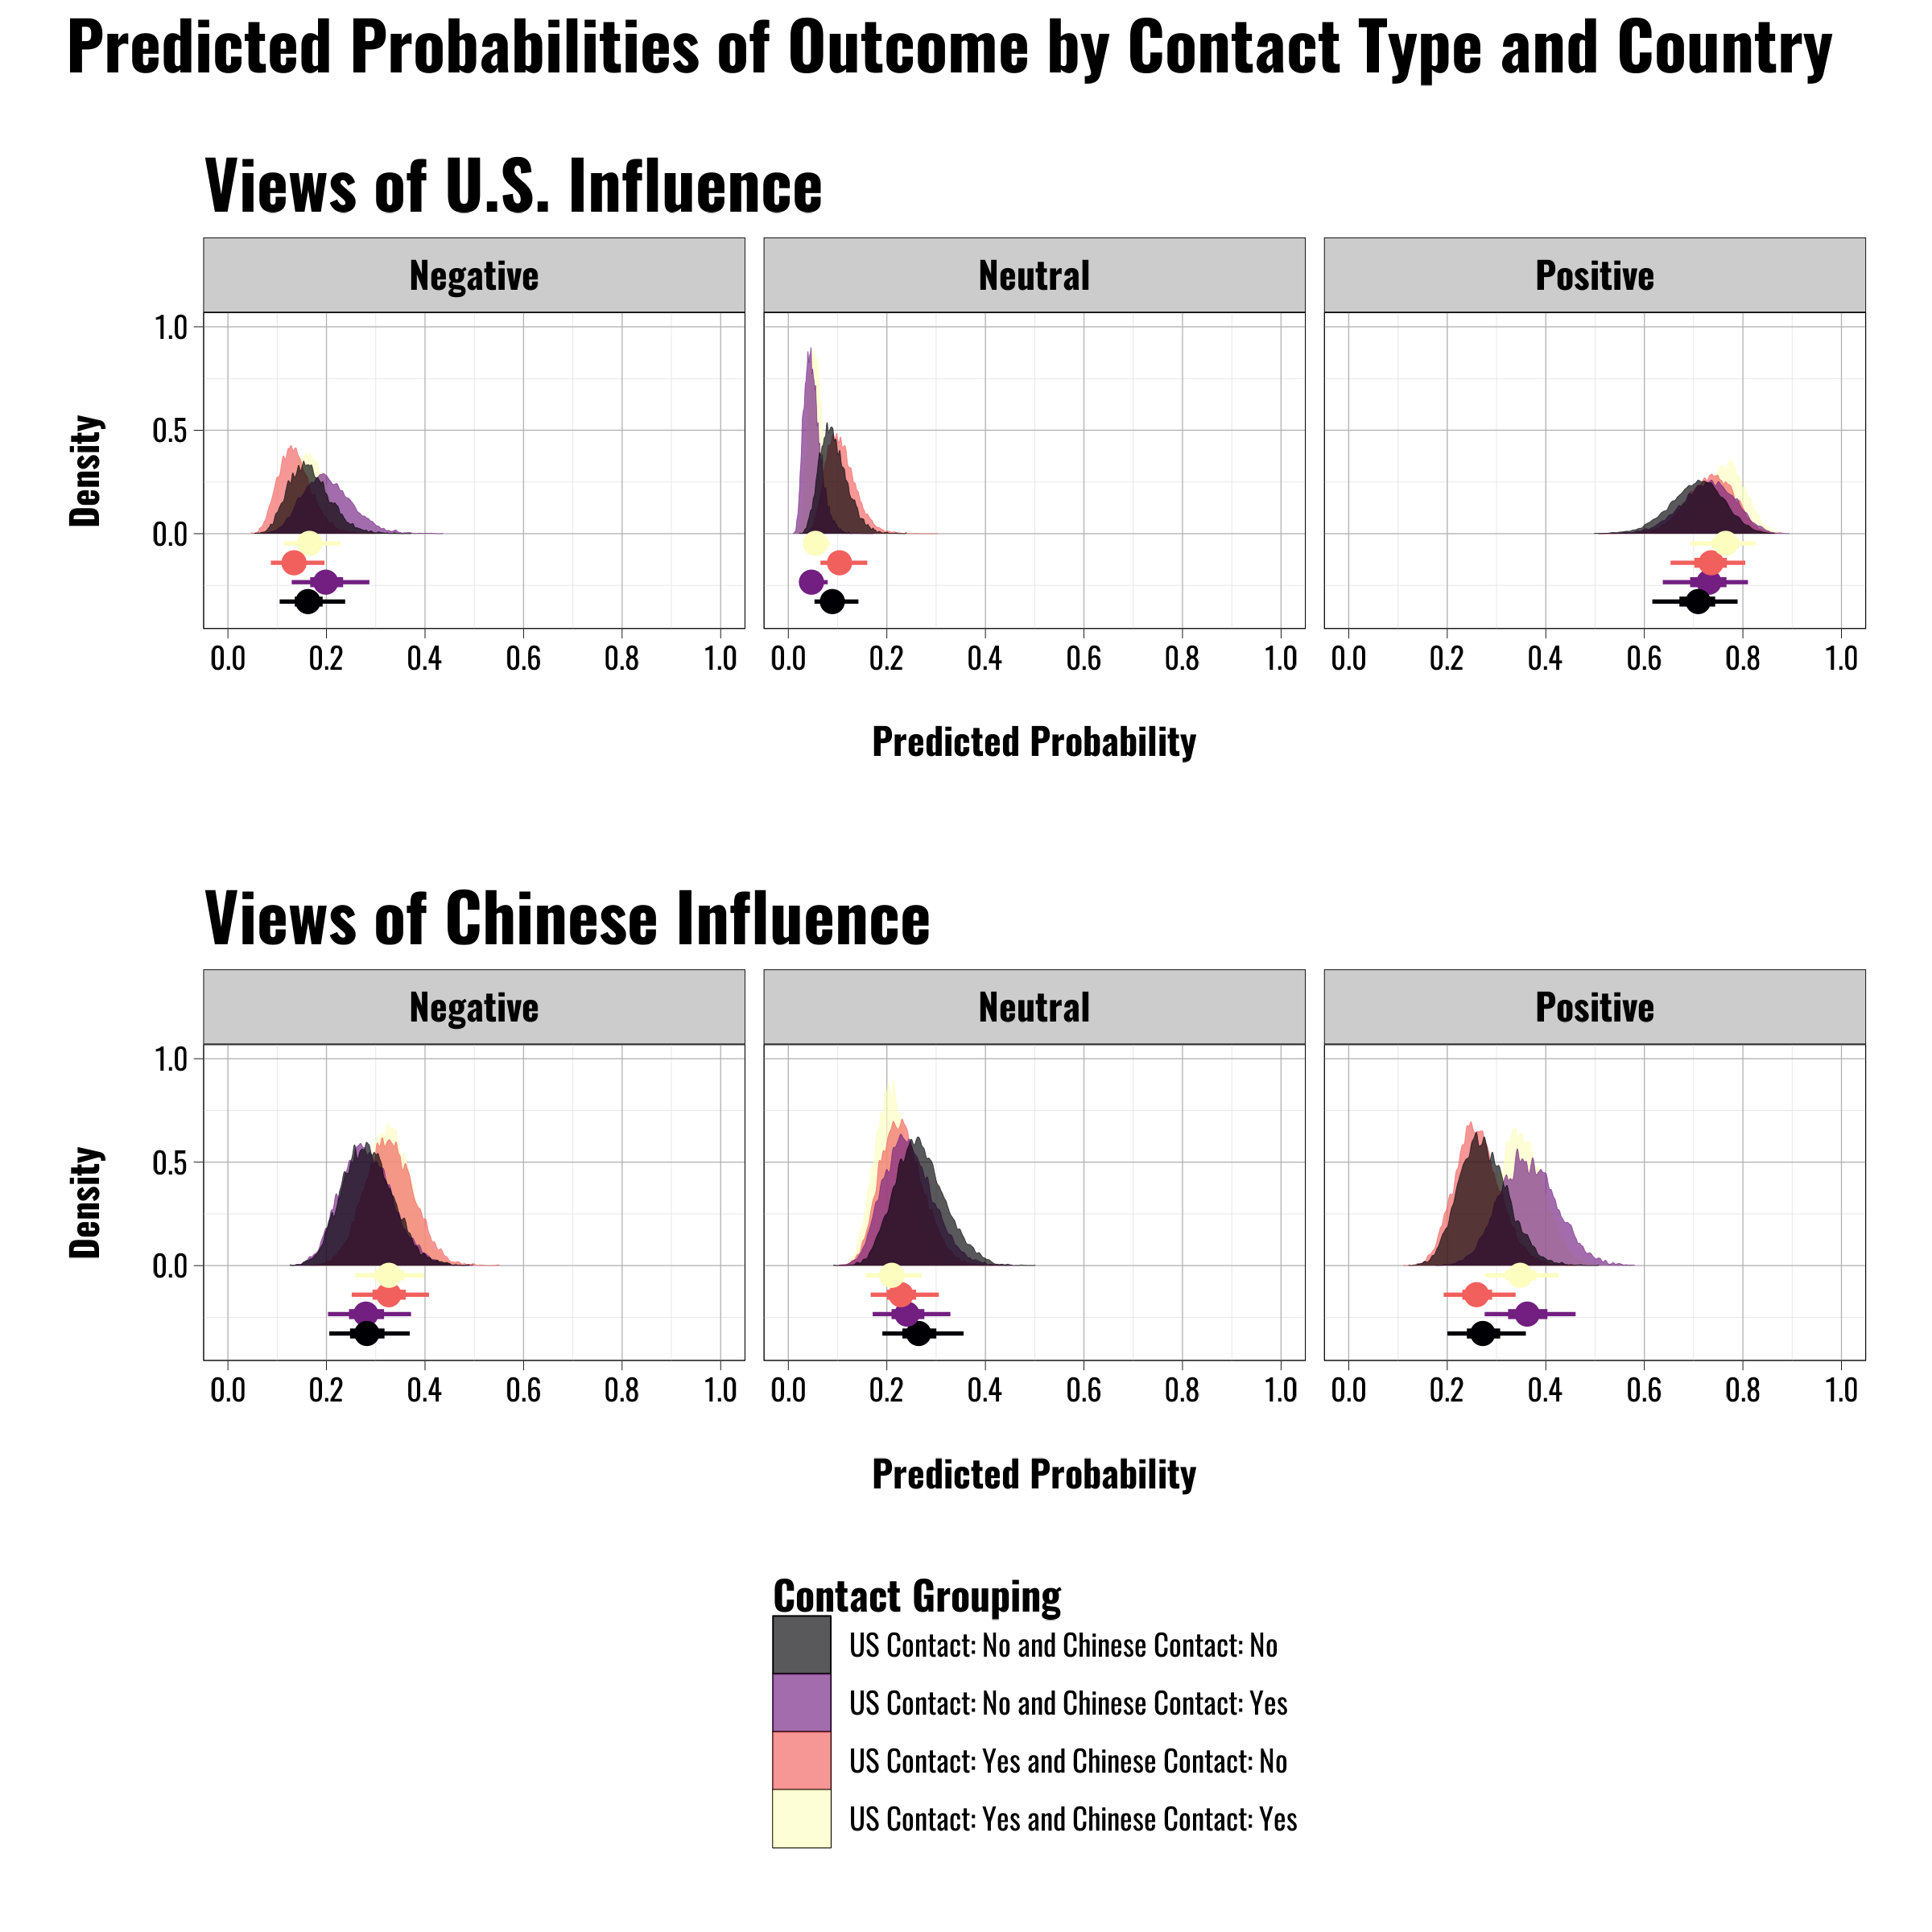
\includegraphics{../../Figures/Kenya-ISA/figure-predicted-probabilities.png}}
		\caption{Multinomial logit coefficient plot for primary variables of interest. \label{pp}}
	\end{center}
\end{figure}

Figure \ref{pp} contains the estimations of our fully specified model when we condition the view of each country's influence on whether they have had contact with individuals from either the United States or China. While there is overlap in these posterior estimations, there is substantive movement in a few cases. In the U.S. influence models, the baseline level of support is very high, making deviation on any graph more difficult as there is less room to go higher on positive and negative views. However, those with U.S. contact are less likely to have negative views and those with Chinese contact are more likely to have negative views. Likewise, those with Chinese contact are less likely to view the United States negatively.

In the Chinese influence models, we see similar movements as well. Those with U.S. contact, but not Chinese contact, are more likely to report negative views of Chinese influence. Those with either contact are less likely to have neutral views on the subject. Finally, Kenyans with exclusively Chinese contact are far more likely to have positive views of Chinese influence. In all six estimations, this last shift is the largest.
